\chapter*{Resumen}
\markboth{RESUMEN}{RESUMEN}

En este trabajo se explica la implementación de Eleven Renderer, un motor de renderizado gráfico de mi autoría, programado en C++ y CUDA desde cero para este TFG. El código fuente se puede encontrar en el repositorio Github \url{https://github.com/101001000/tfg-pathtracer/}. Cuenta con todas las características necesarias para visualizar una escena 3D con relativa eficiencia y hace uso de la arquitectura paralela que ofrecen los aceleradores gráficos. Además se acompaña de una evaluación junto a la justificación de algunas decisiones tomadas durante el desarrollo. A lo largo del trabajo se explonen recursos en caso de querer ampliar información. Así pues, se espera que este trabajo sirva como breve guía y motivación para futuros programadores gráficos.

En este documento también se incluyen las mejoras visuales y optimizaciones aplicadas, junto a varias estadísticas de rendimiento comparando diferentes parámetros. Finalmente se ha puesto a disposición del lector la documentación necesaria para poder crear escenas 3D y visualizarlas de manera fotorrealista con Eleven Renderer, gracias a la posibilidad de importar de manera manual, escenas desde la gran mayoría de software de edición 3D. 

Palabras clave: Renderizado 3D, Path Tracing, Trazado de Rayos, CUDA, Motor Gráfico, Aceleración por GPU.

\chapter*{Abstract}
\markboth{ABSTRACT}{ABSTRACT}

In this work it's explained the implementation of Eleven Renderer, a rendering engine made by me from scratch, coded in C++ and CUDA library, done for this Bachellor Thesis. The source code can be found in the Github's repo \url{https://github.com/101001000/tfg-pathtracer/}. It has all the features needed for 3D scene visualization with relative efficiency and it take advantage of the parallel architecture which graphics accelerators offers. There's also an evaluation for the implementation and the justification of some decisions taken. Some resources are provided in case the reader want in-depth insight about the topic. That been said, it's expected from this work to be used as a small guide and motivation for future developers and graphics programmers.

In this document is also included some visual upgrades and optimizations, accompanied with benchmarks compairing different parametters. Its also offered to the reader, the documentation needed for creating 3D scenes and render it in a photorrealistic way in Eleven Renderer, thanks to the possibility of manually importing scenes from another 3D editing software.

Keywords: 3D Rendering, Path Tracing, Ray Tracing, CUDA, Graphics Engine, GPU Acceleration.


\chapter*{Agradecimientos}
\markboth{AGRADECIMIENTOS}{AGRADECIMIENTOS}

No hubiera sido capaz de realizar este trabajo sólo sin el apoyo de la gente que me ha rodeado a lo largo de estos años de estudio. En primer lugar quiero dar las gracias a mi madre, que aunque no entienda lo que hago, se asegura de que salga adelante. En segundo lugar a mi padre el cual me ha enseñado que el trabajo no es trabajo si te gusta lo que haces. No puedo olvidarme tampoco de mi hermana Violeta, que tengo que quererla.

Por otro lado quiero dar las gracias a Patricia, que ha tenido que aguantar mis cabezazos contra el teclado cada vez que aparecía un error gráfico, y que junto a Hizán, han leído pacientemente mi trabajo y me han ayudado a expresar mejor el caos que tengo por cabeza.

Además quiero dar las gracias a Jorge que ha escuchado con interés el desarrollo de este trabajo y que ha servido como combustible para mi motivación. A él se suman Dani, Jorge, Guille y Alex, que me han acompañado en la carrera y que sin ellos, los cuatro años de carrera no hubieran sido los mismos.

Por último quiero también dar las gracias a mi tutor Carlos, que me enseñó los fundamentos de la computación en paralelo y nos propuso prácticas relacionadas con el procesamiento de imágenes. Aunque no se lo haya dicho, para mí, ha sido muy importante poder realizar trabajos relacionados con la computación gráfica, la que espero que sea mi futura carrera profesional.


\newpage

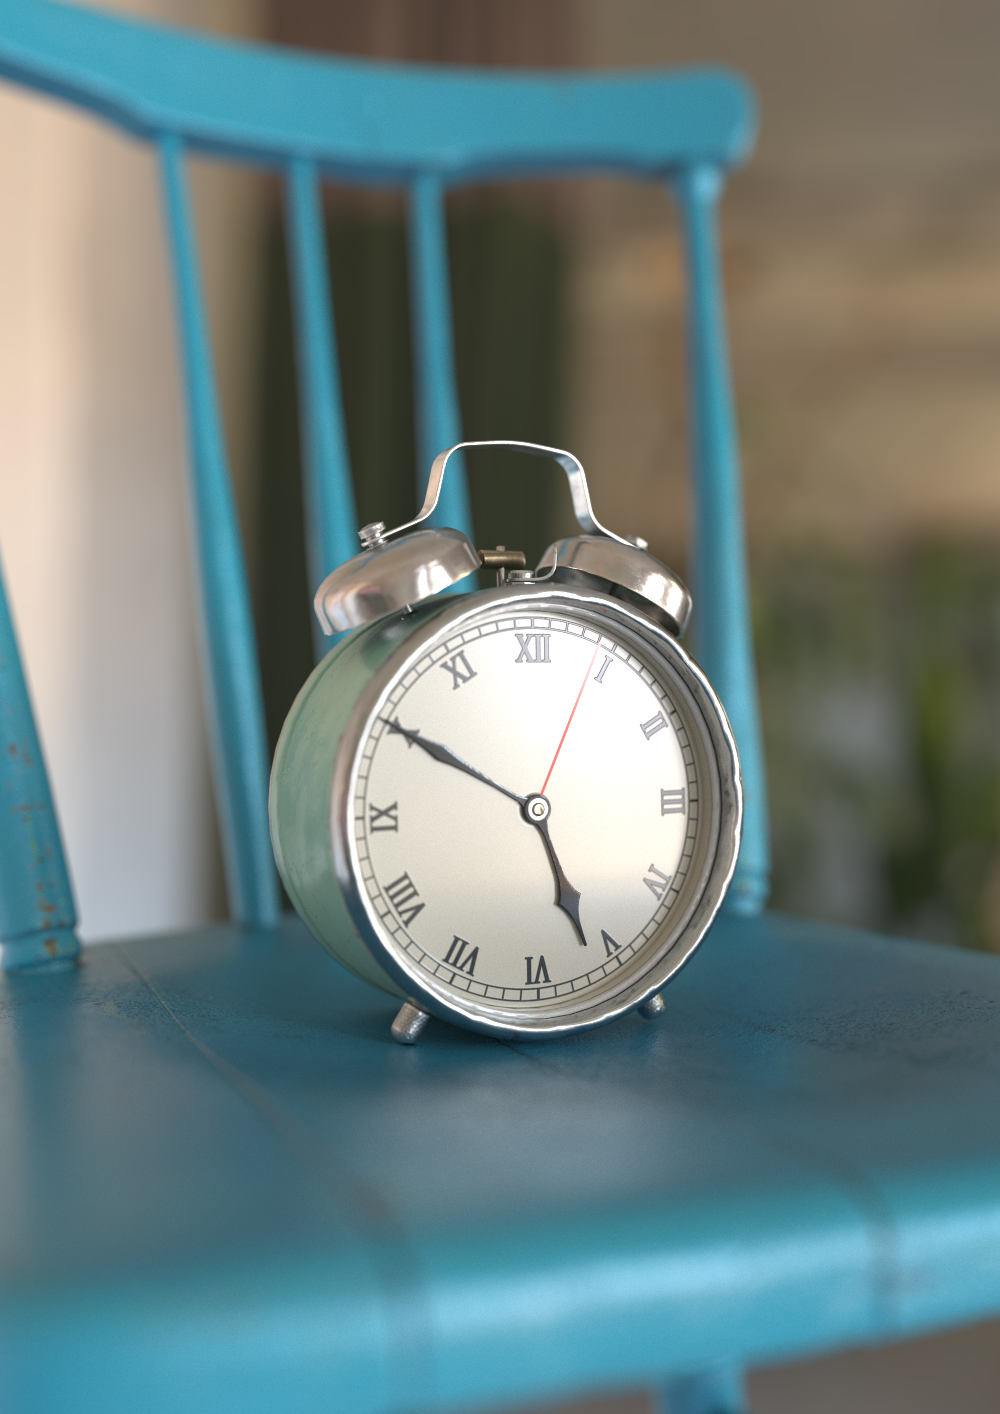
\includegraphics[
    width=1.45\textwidth,
    height=2\textwidth,
    align=t,
    smash=br,
    vshift=4cm,    
    hshift=-4.1cm
]{portada}

\scalebox{5}{\color{white}{Eleven Renderer}}

